\documentclass[a4paper,12pt]{report}
\usepackage[serie,niveau={1MA1},nfiche={}, annee={Emilie-Gourd, 2024--2025}, auteur={ns},theme={Série 9}]{packages/bandeaux}
\usepackage{packages/boites}
\usepackage{packages/fontes}
\usepackage{packages/courslatex}

\begin{document}
{\bfseries Lundi $\longrightarrow$ ex. 1,2,3,4,5  \hfill Jeudi $\longrightarrow$ ex. 6,7,8}

\textLigne{Exercices}

\begin{exo}[1]
Résoudre les équations dans $\mathbb{R}$.
\begin{tasks}(2)
\task $2 \sqrt{3} \cdot x=\sqrt{3} \cdot x-1$
\task $\sqrt{3}-x=\sqrt{2} \cdot x+2$
\task $\sqrt{3}-3 x=\sqrt{2} \cdot x+\sqrt{2}$
\task $\sqrt{2} \cdot x-\sqrt{2}=1-\sqrt{2} \cdot x$
\end{tasks}
\end{exo}

\begin{exo}[1]
	Il s'agit de partager 2100 francs entre trois personnes de manière que la première ait le quart de la part de la troisième et 120 francs de plus que la deuxième.
	\begin{tasks}
		\task Voici trois façons de commencer. Compléter chacune de ces possibilités en fonction de $x$.

\begin{tabular}{|c|c|}
\hline part de la 1re personne~: & $x$ \\
\hline part de la 2e personne~: & \\ 
\hline part de la 3e personne~: &\\ 
\hline
\end{tabular}
\begin{tabular}{|c|c|}
\hline part de la 1re personne~: & \\
\hline part de la 2e personne~: & $x$ \\ 
\hline part de la 3e personne~: &\\ 
\hline
\end{tabular}
\begin{tabular}{|c|c|}
\hline part de la 1re personne~: &  \\
\hline part de la 2e personne~: & \\ 
\hline part de la 3e personne~: &$x$\\ 
\hline
\end{tabular}
\task Résoudre ce problème.
	\end{tasks}
\end{exo}

\begin{exo}[2]
Ayant reçu un héritage, je dépense 2000 francs pour acheter une moto et je place les deux tiers du reste à la banque. Il me reste alors $30 \%$ du montant total de l'héritage. Quel était ce montant?
\end{exo}

\begin{exo}[2]
 Le rectangle représenté cí-dessous a été découpé en 5 carrés. Le périmètre du rectangle est de 1 m . Déterminer son aire.
\begin{center}
	\begin{tikzpicture}[scale=0.5]
    \tkzDefPoint[label=below:{}](0,0){A}
    \tkzDefPoint[label=right:{}](0,2.25){B}
    \tkzDefPoint[label=above:{}](0,4.5){C}
    \tkzDefPoint[label=above:{}](-2.25,4.5){D}
    \tkzDefPoint[label=above:{}](-5.25,4.5){E}
    \tkzDefPoint[label=above:{}](-5.25,1.5){F}
    \tkzDefPoint[label=above:{}](-5.25,0){G}
    \tkzDefPoint[label=above:{}](-3.75,0){H}
    \tkzDefPoint[label=above:{}](-2.25,0){I}
    \tkzDefPoint[label=above:{}](-2.25,2.25){J}
    \tkzDefPoint[label=above:{}](-2.25,1.5){K}
    \tkzDefPoint[label=above:{}](-3.75,1.5){L}
\tkzDrawPolygon(A,B,J,I)
\tkzDrawPolygon(B,C,D,J)
\tkzDrawPolygon(D,E,F,K)
\tkzDrawPolygon(F,G,H,L)
\tkzDrawPolygon(H,I,K,L)
 \end{tikzpicture}
\end{center}
\end{exo}
\begin{exo}[1]
Un problème de Leonhard Euler (1707 - 1783).

Un père mourut en laissant quatre fils. Ceux-ci se partagèrent ses biens de la manière suivante : le premier prit la moitié de la fortune, moins 3000 livres; le deuxième en prit le tiers moins 1000 livres; le troisième prit exactement le quart des biens; le quatrième prit 600 livres plus le cinquième des biens. Quelle était la fortune totale, et quelle somme reçut chacun des enfants?
\end{exo}

\begin{exo}[1]
Trouver deux nombres entiers consécutifs tels que le quart du premier ajouté au cinquième du plus grand donne 29.
\end{exo}

\begin{exo}[1]
Sur le dessin ci-dessous, la figure ombrée est un carré, et le grand quadrilatère, un rectangle.

(Toutes les longueurs sont en cm.)

\hfill
\begin{minipage}[t]{0.5\textwidth}{
\vspace{0pt}
\begin{tikzpicture}
    \tkzDefPoint[label=below:{}](-1,-1){A}
    \tkzDefPoint[label=right:{}](-1,1){B}
    \tkzDefPoint[label=above:{}](2,0.5){C}
    \tkzDefPoint[label=above:{}](3,0.5){D}
    \tkzDefPoint[label=above:{}](2,-1){G}
    \tkzDefPoint[label=above:{}](3,1){E}
    \tkzDefPoint[label=above:{}](3,-1){F}

    \tkzDrawPolygon(A,B,E,F)
    \tkzDrawPolygon(F,G,C,D)
    \tkzFillPolygon[pattern=north west lines](F,G,C,D)
    \tkzDrawSegment[dashed,dim={$2$,15pt,right=2mm,midway,font=\footnotesize}](E,D)
    \tkzDrawSegment[dashed,dim={$x$,-15pt,right=2mm,midway,font=\footnotesize}](F,D)
    \tkzDrawSegment[dashed,dim={$6$,-15pt,below=2mm,midway,font=\footnotesize}](A,G)


\end{tikzpicture}
}
\end{minipage}
\begin{minipage}[t]{0.4\textwidth}{
\vspace{0pt}
Déterminer $x$ pour que l'aire de la partie blanche soit égale à $38 \mathrm{~cm}^2$.
}
\end{minipage}

\end{exo}
\newpage
\begin{exo}[3]
 Résoudre les équations dans $\mathbb{R}$.
	\begin{tasks}(3)
\task $(2 x-3)^2=(7 x+3)^2$
\task $12 x-9 x^2=4$
\task $4 x(x+1)=-1$
\task $9 x^2-27=0$
\task $\dfrac{1}{\sqrt{2}}(5 x-7)=\sqrt{2} x+\sqrt{18}$
\task $x^2+4 x=32$
\task $4(x-7)=x^2(x-7)$
\task $x^3-2=x(2 x-1)$
%\task $x^2+6 x+3=0$
	\end{tasks}
\end{exo}

\textLigne{Entraînement individuel}
\begin{exo}
Factoriser le plus possible.
	\begin{tasks}(3)
\task $4 x^4-4$
\task $x^3-x^2-4(x-1)$
\task $16 x^4-9 y^2$
\task $3 x^2+6 x-24$
\task $8 x^3-8 x^2+2 x$
\task $(x+y)^2-4 u^2$
\task $x^3-5 x$
\task $x^4-64$
\task $4 y^2-12 y+9$
\task $a^2-a b-a+b$
\task $(4 x-1)^2-9(3-x)^2$
\task $4 a x^2 y^3-(a x y)^2+5 b x^3 y^2$
	\end{tasks}
\end{exo}
\begin{exo}
Résoudre les équations dans $\mathbb{R}$.
	\begin{tasks}(2)
\task $2\left(\dfrac{x}{3}+3\right)=0$
\task $\dfrac{1-6 x}{4}=2\left(1-\dfrac{3}{4} x\right)$
\task $3 x=\dfrac{x-55}{6}$
\task $x+\dfrac{1}{4}=-\dfrac{3}{7}$
	\end{tasks}
\end{exo}
\end{document}
